%Edit 0026 ZZZ to report number nnnn 
%Edit 3.3.3 YYMILE to milestone number m.m.m
%Edit Design patterns evaluation report YYTITLE to report title - Words Start with Caps
\documentclass[11pt,twoside,a4paper]{article}
%%======================================================================
%% PACKAGES:
%%
%\usepackage{times}               % Times+Helvetica+Courier fonts
\usepackage{helvet}              % helvetica + cmr
\usepackage{fancyhdr}       % package for headers/footers
\usepackage{amsmath}
\usepackage{amssymb}
\usepackage{graphicx}            % Graphics.
%\usepackage{a4}                  % page layout to fit A4
%\usepackage{lastpage}            % get page no of last page
%\usepackage{ifthen}              % logical branching
\usepackage{hyperref}            %insert hyper-links
\usepackage{latexsym}
% uncomment the following to override auto page total
%\pptotal{20}
%%======================================================================

% ensure sans-serif font used throughout
\renewcommand{\familydefault}{\sfdefault}

\newcommand{\culhamissueno}{1.00}%<==edit
\newcommand{\culhamshorttitle}{CD/EXCALIBUR-FMS/0031}%<==edit
\newcommand{\Sec}[1]{Section~\ref{sec:#1}}
\newcommand{\Fig}[1]{Figure~\ref{fig:#1}}
\newcommand{\Tab}[1]{Table~\ref{tab:#1}}
\newcommand{\Eq}[1]{Equation~(\ref{eq:#1})}
\newcommand{\Eqs}[2]{Equations(\ref{eq:#1}) and~(\ref{eq:#2})}
\newcommand{\Figs}[2]{Figures~\ref{fig:#1}--~\ref{fig:#2}}
%Bold lc for script names, tt for computer code and file-names
%\F{NEPTUNE} always in caps
\newcommand{\F}[1]{\textsc{#1}}
\newcommand{\B}[1]{\textbf{#1}}
\newcommand{\T}[1]{{\tt #1}}
\newcommand{\V}[1]{\mathbf{#1}}
\newcommand{\I}[1]{\textit{#1}}
\newcommand{\nep}{\textsc{NEPTUNE}}
\newcommand{\exc}{\textsc{E}x\textsc{CALIBUR}}
\newcommand{\Papp}{Proxyapp}
\newcommand{\papp}{proxyapp}



%%======================================================================

%% REPORT COVER PAGE Information

\newcommand{\culhamtitle}{\LARGE Select techniques for MOR (Model Order Reduction)  \\[1.0\baselineskip] M2.5.1 }%<==edit

%%QA BOX information -- change following as needed
\newcommand{\culhamboardname}{Martin O'Brien}%<==edit
\newcommand{\culhamcontactname}{Rob Akers}%<==edit
\newcommand{\culhamauthor}{Wayne Arter}%<==edit
\newcommand{\culhamauthora}{Ed Threlfall}%<==edit
%\newcommand{\culhamcontacttel}{Telephone: 01235 466498}
%\newcommand{\culhamcontactemail}{Email: rob.akers@ukaea.uk}

\newcommand{\culhamdate}{15 March 2021}%<=edit
\newcommand{\culhamdatea}{15 March 2021}%<=edit
\newcommand{\culhamdateb}{15 March 2021}%<=edit

% reproduce Rob's page size

\setlength{\textheight}{220.0mm}
\setlength{\textwidth}{165.0mm}
\setlength{\topmargin}{0.0mm}
\setlength{\oddsidemargin}{0.0mm}
\setlength{\evensidemargin}{\oddsidemargin}
\setlength{\parindent}{0mm}
\addtolength{\parskip}{0.5\baselineskip}
\setlength{\topsep}{0pt}
\setlength{\itemsep}{0pt}

%%======================================================================
\begin{document}

%Titlepage comes out wrong size, but should look right apart from
% picture which cannot be wider than c.150mm.
% To produce conforming report rp1pub.pdf
% remove title page by commenting out lines ending in %<==omit, then
% sed -e '/<==omit$/s/^/%/' < rp1.tex > rp1omit.tex
% pdflatex rp1omit;bibtex rp1omit; pdflatex rp1omit
% pdfunite cover.pdf rp1omit.pdf rp1pub.pdf 
\begin{titlepage}%<==omit
\vspace*{-30mm}%<==omit

\includegraphics[width=2.5cm]{../corpics/cofaplus} \\[2.0\baselineskip]%<==omit
{\LARGE {\textbf{\textsf{ExCALIBUR}}}}\\[2.0\baselineskip]%<==omit
{\LARGE \culhamtitle } \\[2.0\baselineskip]%<==omit
{\textbf{\textsf{Abstract}}}\\%<==omit
The report describes work for \exc \ project \nep \ %<==omit
at Milestone 2.5.1. %<==omit
Report on the status of programming models and code generators for the
various node architectures focused on performance, usability, maintainability
and  availability.  
%ed%<==omit
%<==omit
\vfill%<==omit
\centerline{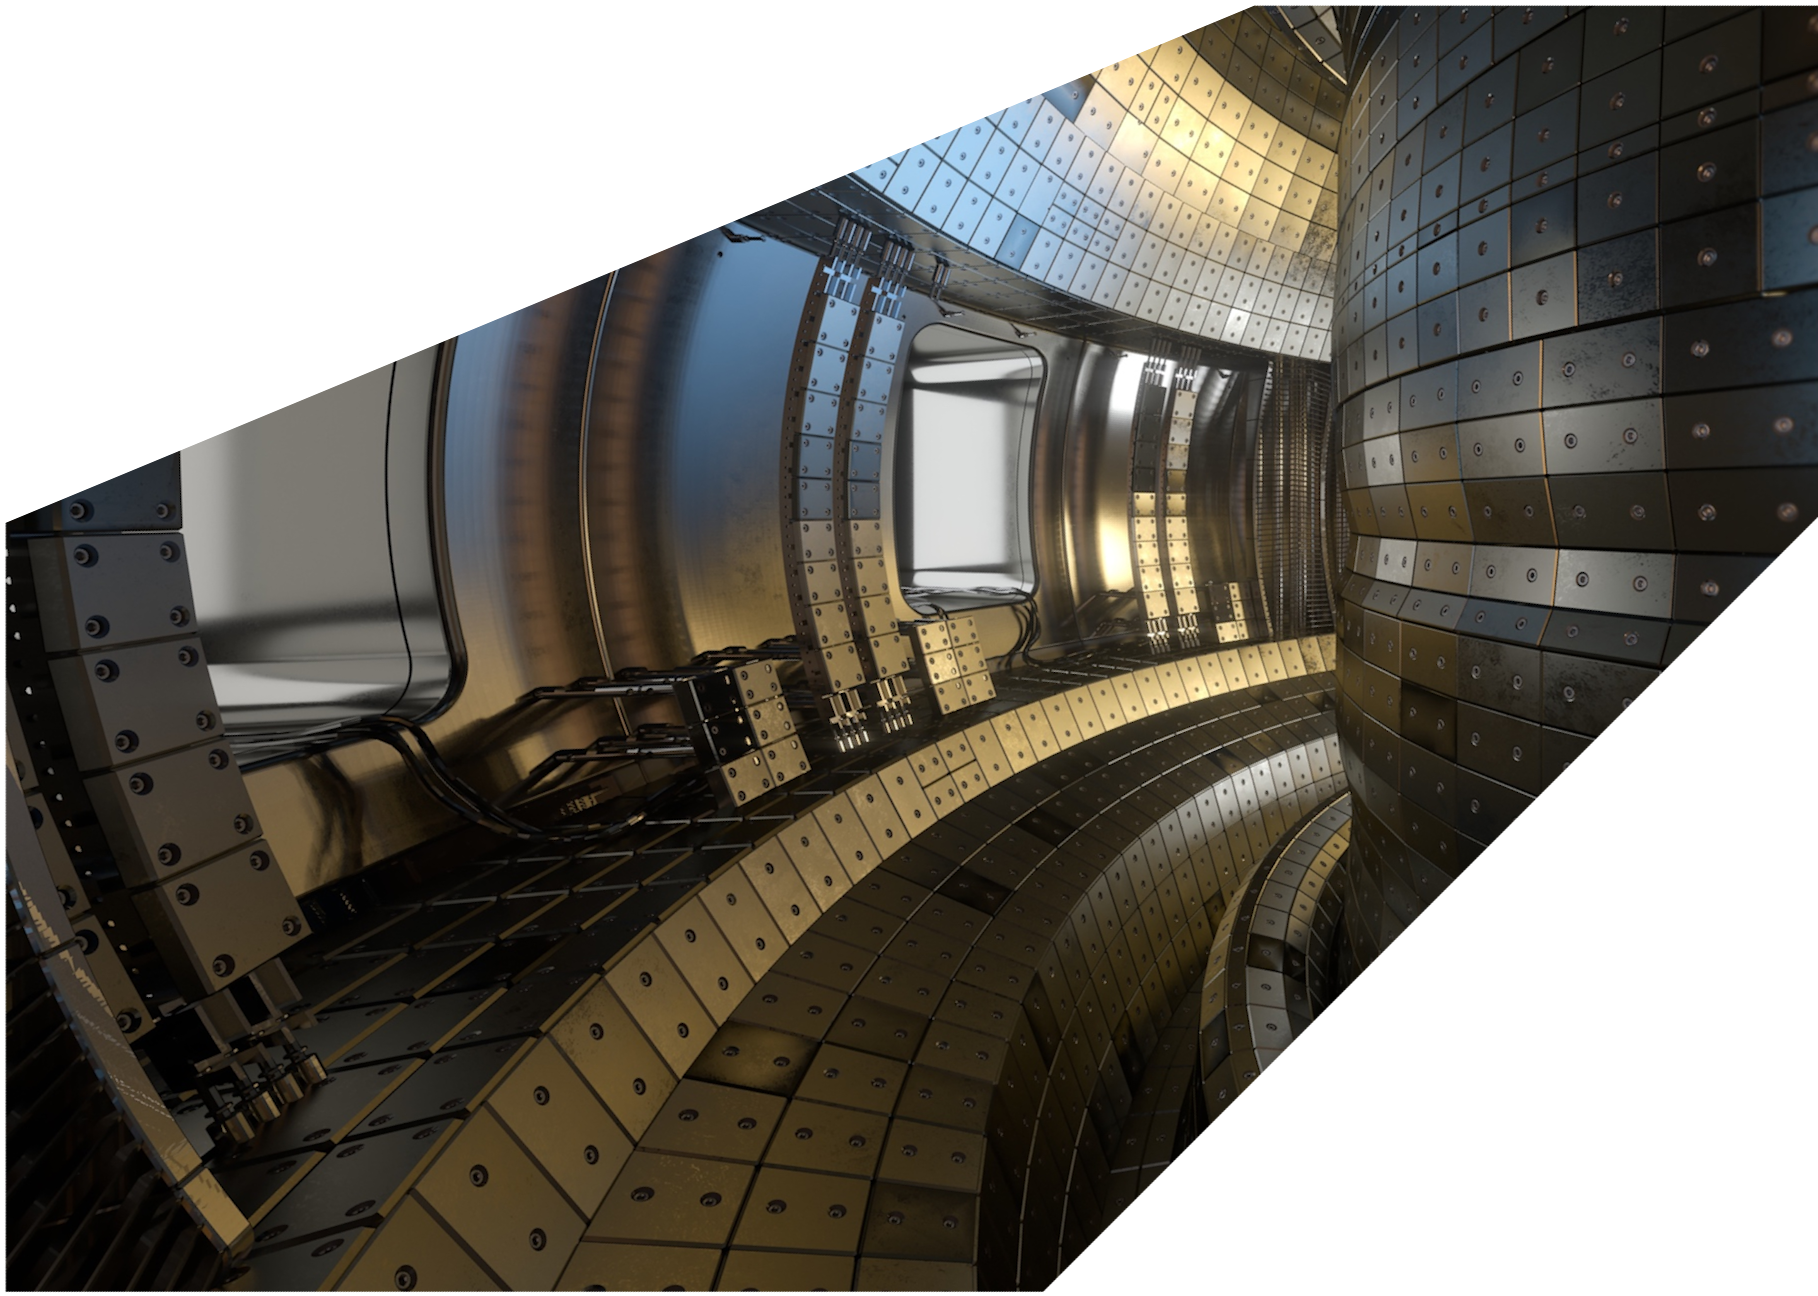
\includegraphics[width=0.9\textwidth]{../corpics/tokintcrop}}%<==omit
\end{titlepage}%<==omit

\hspace{-30mm}\begin{table}[h]
\sffamily
\begin{center}
\textbf{\textsf{UKAEA REFERENCE AND APPROVAL SHEET}}
\begin{tabular}{||p{5.7cm}|p{4.7cm}|p{5.0cm}||}
\hline
\hline
& Client Reference: &  \\
\hline
& UKAEA Reference: & \culhamshorttitle \\
& & \\
\hline
& Issue: & \culhamissueno \\
\hline
& Date: & \culhamdateb \\
\hline
\multicolumn{3}{||l||}{} \\
\multicolumn{3}{||l||}{Project Name: ExCALIBUR Fusion Modelling System} \\
\multicolumn{3}{||l||}{} \\
\hline
\end{tabular}
\begin{tabular}{||p{3.3cm}|p{4.6cm}|p{3.5cm}|p{3.6cm}||}
\hline
& Name and Department & Signature & Date \\
\hline
Prepared By: & \culhamauthora & N/A & \culhamdate \\
& \culhamauthor & N/A & \culhamdate \\
%& \culhamauthorb  & N/A & \culhamdate \\
%& \culhamauthorc  & N/A & \culhamdate \\
& & & \\
& BD & & \\
\hline
Reviewed By: & \culhamcontactname & 
\includegraphics[width=3.0cm]{../corpics/blanksign}& \culhamdatea \\
& & & \\
& Advanced Computing Dept. Manager & & \\
\hline
%Approved By: & \culhamboardname  & \includegraphics[width=3.0cm]{../corpics/mobsign} & \culhamdateb \\
%& & & \\
%& MSSC & &\\
%\hline
\hline
\end{tabular}
\end{center}
\end{table}
%ed

\clearpage
\section{Introduction}\label{sec:intro}
This report collates technical material used to inform the preparation of the call for 
procurement of support for Uncertainty Quantification~(UQ).
The work performed primarily consisted of collating material produced
internally~\cite{y2re241,y2re242,y2re251,y2re313}
and by external grantees at UCL~\cite{2047352_1-TN-01,2047352_2-TN-01}, plus
hands-on exploration of sampling techniques, the construction of surrogates and the study
of dimensionally reduced models.
The production of this call reflects the importance attributed to UQ in project \nep, so that 
the software produced should be capable of producing `actionable' results, that could form a significant
input to multi-million pound procurements.

It seems worthwhile to start by recapitulating the project
\nep \ requirements for UQ, insofar as they are currently understood. In particular, to
note a clear distinction between the experiments that \nep \ code needs to model, and the
outputs of the simulations themselves.  Relevant experiments are almost entirely medium-sized
and large tokamaks, where it seems that even the edge plasma has a temperature of
around~$10$\,eV~($10^5$\,K). The presence of magnetic fields of order $1-10$\,T, and
electric fields of around $10^4$\,Vm$^{-1}$ implies a hostile environment, subject further
to large electromagnetic transients not just at start-up and ramp-down of a discharge, but also caused by
plasma instabilities such as ELMs and sawteeth.  Most diagnostics struggle to achieve absolute
accuracies of $10$\,\%, although they usually detect the direction of smaller changes reliably.
Many are ``one-of-a-kind" so require careful interpretation, and all signals may have been subject to
filtering both at low and high frequencies, to remove  `spikes' and `drift'.
In comparison, signals from simulation are very `clean', but the simulation may lack
crucial realism, in that either important physical processes are not treated or 
if included, that the spatio-temporal discretisation may not be sufficiently fine to
represent them accurately.

%The Model  expt. - noisy, large unc. toks
%simulation - clean, level of detail controllable by mesh refinement, more detailed physics

Turning to the expected usage of the \nep \ software, this covers  both physics and engineering.
Both physicist and engineers are potentially interested in everything computed by the software, which is of course
likely to be an overwhelming amount of detail. A physicist is more likely to begin by
formulating simpler models and use the software to determine their appropriateness and accuracy,
an engineer probably more likely to use the output of simulation as a basis for producing simplified models.
An experimental physicist may be satisfied with qualitative accuracy, provided it is obtained
rapidly enough to help formulate the next experimental `shot' (eg.\ by indicating that more
or less gas input would be helpful), whereas a more theoretical
%counterpart may want a model useful for extrapolation to reactor parameters. An engineer
counterpart may want to quantify the difference between model predictions and experiment 
sufficiently well to help produce a more refined model. An engineer
seeking to design a reactor may be interested only in a relatively small number of
quantities of interest~(QoI) but which need to be determined more precisely, 
such as local maxima in time-averaged heat flux, whereas
other engineers may see edge code as forming a part of a digital twin, to be used to help control
operation of an actual tokamak device where accurate time-dependent modelling will also be critical.
%Users physicist -  formulate simpler models useful for extrapolation of geometry and parameter changes
%potentially interested in everything as extrapolation
%experimental physicist, qual accuracy OK for fuelling
%engineering design - few QoI, static
%digital twin (as part) - for operation and control, quant accuracy, time dep.
It is notable that most of the preceding requirements involve extrapolation,
from model to new features of an existing experiment or, in the design case, to more
extreme values of geometrical size, magnetic field etc. representing a fusion reactor
relative to existing experiments such as JET.
%Requirements - interpolation, to obtain sufficient data to perform to a given accuracy
%extrapolate - "to expt" and to new parameters

For the above it is therefore as Smith~\cite{smithUQ} describes (see also the \nep \
report~\cite[\S\,1]{y2re313}), important that UQ involves more than just clever sampling
to identify parameter sensitivities, and the standard definitions of ways of quantifying
these such as Sobol indices~\cite{y2re241}. In particular,
the production of surrogate models is within scope of UQ.
%sampling imp. for identifying important parameters
It is worth saying that in one sense even the most complex partial differential equation~(PDE) models of plasma are 
simply surrogates for experimental `reality'. The most detailed and least controversial
model of tokamak plasma consists in treating it as of order~$10^{20}$ or more particles evolving
under the influence of external and self-generated electromagnetic fields, but
this is of course not tractable even at the Exascale~\cite{Wa95a}, without very selective
sampling of the particles. Currently, particle models are seen as at best struggling to capture
edge plasma behaviour, with no certain likelihood of significant improvement, and 
in any event there is a separate calls that could cover research into particle sampling. The PDE models
attempt to capture the key physics of the plasma particles, viz.\ their appearance, motion,
interactions with other particles and eventual loss, as terms representing respectively
source, advection, diffusion and sinks in continuum models. Unfortunately, long mean free
paths~(\emph{mfp}s) mean that at least in some regions it is necessary explicitly to represent
phase-velocity dependence of plasma density, and the resulting basic 6-D dependence of 
fields (5-D if gyro-averaged models are used) stretches current and foreseen computing
facilities. In any event, above applications eg.\ preliminary design studies and operational control,
require models capable of evaluation within seconds or less, ie.\  surrogates for the
PDEs, expected to have lower spatial dimensionality (2-D or 1-D) or even as systems of 
ordinary differential equations~(ODEs).
%Surrogate. PDE solution as surrogate for expt/reality, advection, diffusion, sinks and sources.

Unfortunately for application to \nep, most surrogates have been designed for use as
interpolants. Nonetheless, interpolation is likely to be important at least within the software,
eg.\ to connect different models, and the book by de~Boor~\cite{deboor} has interesting
material relating to the use of splines in this context. In particular, de~Boor lists
theorems relating to the optimality of spline polynomial interpolation, so that there might be
wonder that any other form of interpolation is required. In fact, spline optimality is found only in 
the energy or least-squares norm, so there is anyway the possibility of fitting the data
with polynomial functions that have under- and over-shooting oscillations between sample
points (called nodes in spline jargon). Moreover, de~Boor illustrates the potential for dramatic failings
using what he refers to as the Titanium heat data set~\cite[Fig.\ XIII.1]{deboor}. The data is
a set of some~$50$ apparently regularly spaced samples of a function which is practically
flat except for one distinct `hump', rising to four times the value of the `plateau' over
c.\ $15$\,\% of the range. Since the interpolation is by a piecewise  ($5^{th}$ order polynomial)
the undershoot by greater than the maximum `hump' value is in many respects more impressive than
that exhibited in Boyd's book~\cite[Fig.\ 4.3]{boyd} as part of his demonstration of the Runge
phenomenon, ie.\ that polynomial interpolation at evenly spaced points may diverge. In both books,
the problem is identified as due to poor choice of sample points. de Boor~\cite[Fig.\ XIV.5]{deboor}
shows improved fitting if the number of samples in the plateau region of the \emph{Ti} heat data is reduced,
whereas Boyd points out that optimal $N^{th}$~order polynomial interpolation is achieved using
sample points that are the roots of the Chebychev
polynomial of degree~$(N+1)$, that cluster as close together as~$1/N^2$ near the end-points
of the sample region. In any event, for many interpolation purposes, it seems that polynomial spline
fitting with an order of three or so, is adequate \emph{provided} the nodes are chosen suitably. The cost
scales as the operation count  of a banded-diagonal matrix solver, so~$\mathcal{O}(N)$ where $N$~is the
number of points to be interpolated per dimension.
There are however strong proponents for the use of rational polynomial interpolation~\cite{stoerbulirsch}
and in particular radial basis function~\cite{fornbergflyer}. Wavelet bases~\cite{Fa15Wave} also
have their adherents, and special conditions such as periodicity or infinite domain mean that
respectively Fourier series and the Hermite basis are to be preferred. The Hermite basis is
employed in the Polynomial Chaos Expansion~(PCE), which is advocated by P.\ Coveney~et~al, see
the \nep\ report~\cite{2047352_1-TN-01}. % and special bases will not be discussed further

Accurate spline fitting requires a sufficient amount of data to enable best location of the
nodes, which, since they generally aim to use as few nodes as possible, is commonly unavailable
in the output of
highly expensive numerical calculations. This lack of data means also that interpolation using
Neural Networks~(NNs)  is mostly unsuitable, and motivates the use of Gaussian Processes~(GPs)
for interpolation despite their expense, that~$\mathcal{O}(N^3)$ of inverting a full matrix~\cite{y2re242}.
They come with the benefit of accompanying error bounds, and seem to be relatively stable when
used for extrapolation~\cite{Ch20priv}. They may be very effective in combination with a 
special basis produced by Principal Component Analysis~(PCA), \emph{aka} Proper Orthogonal Decomposition
or POD, see the \nep\ report~\cite{2047352_2-TN-01}. Moreover, S.~Guillas~\cite{Li17Dime} describes
a number of techniques which outperform PCA, in particular favouring a reproducing kernel
approach to estimating derivatives needed to optimise the basis. This is coupled with
a sequential approach to selecting sample points.
Indeed, choosing sample points appropriately is still a major issue for GPs, which P.~Challenor (private
communication) has explored extensively and favours `Leave One Out'~(LOO).

% as interpolant (1) polynomial spline, GP, NN.
%limitations of spline, GP and NN in table/appendix.
%De Boor for spline, Ti heat data XIII.1 - Gibbs like phena - but XIV.5 shows OK if get nodes
%in right place
Nonetheless, given the general need for extrapolation, it is desirable to incorporate as much
physical knowledge as possible into the surrogate model. The hopes are that the parameters
of the surrogate are either invariant under the extrapolation, or that they have well-determined
scaling properties, and that all important physical processes have been identified.
The parameters of the surrogate may then be fitted using existing data from
experiment and/or simulation as described above.
The surrogate may need to be space and/or time dependent as required by the
user and application. Of course, such surrogates can be very useful for interpolation also.
Worthy of particular mention is Model Order Reduction~\cite{y2re251}, which for linear and some nonlinear
problems, offers reliable estimates of error in interpolating Quantities of Interest~(QoI),
hence likely to be particularly useful for the design engineer.

The body of the current document consists of hands-on exploration of sampling techniques
in \Sec{bout}, the construction of surrogates by Gaussian Processes in \Sec{nektar} and
of surrogates consisting of dimensionally reduced models in \Sec{dimred}.
The implications for the call are summarised in \Sec{summ}.
%ed
\clearpage
%\section{Task Work}\label{sec:taskwork}

\section{{\nep\  Meeting: 22 April 2021 10.15-10.45am BST}}

\emph{Present}

\begin{itemize}
\item Chair: Wayne Arter, UKAEA
\item Ed Threlfall, UKAEA
\item Vassil Alexandrov, STFC
\item Sue Thorne, STFC

\end{itemize}

\section{Minutes}

WA presented the agenda: to go through the most recent report received from STFC, to 
discuss STFC's work since the submission of that report, and to conclude with a 
general discussion about proposed work going forward. The `01'~report~\cite{2047353-TN-01}
was not discussed.

WA thanked ST and VA for their most recent `02' report~\cite{2047353-TN-02}, noting that this 
meeting included only two of the four authors named on the report.  WA praised 
the report as a useful introduction, then noted that it was useful to have 
received also the \LaTeX\ source which allows UKAEA to make minor notational 
corrections.  WA had a slight issue with some of the syntax in the report, 
taken from a textbook to which he had no access (something like 
$diag(\mathcal{L}_x \left ( \phi \right ))$, with the confusion being that the 
diagonal of the matrix would be zero for a centred-difference scheme.  However, 
WA requested no changes to the report.  Another question WA had concerned 
S.3.4, which mentioned other libraries of interest but which did not include 
direct sparse solvers.  ST answered that this section was concerned only with 
preconditioners and iterative methods - not direct solvers.  WA said he was not 
very familiar with direct solver libraries and asked whether ST was proposing 
to use them as part of a preconditioner; ST replied that she was not, but noted 
that direct solvers could be applied to preconditioner sub-blocks (note Jack 
Dongarra list {\it does} include direct solvers); though indicated that the 
sub-blocks are probably too large for direct methods to be useful.  WA 
concurred - he had expected this to the the case - though noted that there was 
historically a commercial direct-solver electromagnetism code (and cited the 
then-lack of understanding of preconditioners for the high-frequency Helmholtz 
problem).  ST noted that \F{MUMPS} can be used directly or for preconditioning 
(incomplete factorization).  WA concluded this discussion by again commending 
the report.

WA moved on to a discussion of work performed since the submission of the 
report; ST confirmed that work had continued.  WA asked whether STFC planned to 
consider stochastic/Monte Carlo methods; ST and VA replied in the 
affirmative.  ST described current work as having two phases: 
\begin{enumerate}
\item Examining integration of preconditioners with \F{BOUT++} and \F{Nektar++} (Emre Sahin has been 
in contact with David Moxey re. the latter code, though this work has been 
delayed by unavoidable circumstance); the aim is to interface a MCMCMI (Markov 
Chain Monte Carlo Matrix Inversion) preconditioner acting on the entire matrix; 
and
\item  work on blocking, for which ST has developed new theory for a class of 
`non-symmetric constraint preconditioners' (her term) aimed at clustering 
eigenvalues, also trying different families of block factorizations for 
efficient generation of preconditioners.  ST is currently working on narrowing 
down the factorizations to the most useful ones. 
\end{enumerate}
WA acknowledged the challenge 
of the problem including hyperbolics, than agreed that the direction of current 
work was promising.

WA asked whether there was anything else to discuss - ST and VA explained that 
their co-workers Anton Lebedev and Emre Sahin were stuck on other projects, so they intend to 
onboard a new person formerly of Manchester and prior to that Jack Dongarra's 
group (and who has worked with Anton/Emre in the past).  WA acknowledged that 
the shortness of this project was a potential issue and also that the 
Manchester group was very strong (and that UKAEA had tried to entice them onto 
\nep\ , though there will be future opportunity to do so).  ST noted the 
advantage of having a flexible team of people at the Hartree Centre.

WA steered the discussion to work going forward.  ST is working on interfaces 
for \F{BOUT++} and \F{Nektar++} and implementing preconditioning for the core 
test problems supplied by Ben Dudson.  ST plans also to test multigrid methods 
against stochastic / Monte Carlo.  WA confirmed that it was acceptable for STFC 
to abandon any directions they judged to be of less promise (eg.\ direct 
solvers).  ST confirmed this, noting that the future direction toward 
matrix-free implementations was likely to favour hybrid stochastic methods and 
not direct solvers.  WA asked what experience STFC had in domain decomposition 
methods; ST replied that she personally had more of a background in nested 
linear algebra techniques, citing her work with Jennifer Scott in the 
computational mathematics group.  Others at STFC have implemented a domain 
decomposition load balancing for \F{OpenFoam} with new domain decomposition 
algorithms that showed much promise.  VA reminded WA that STFC are finalizing an 
agreement with UKAEA (via Rob Akers) which will allow for wide-ranging 
future collaboration.

WA explained that a major concern of \nep\  is coupling continuum (3-D/5-D) to 
particle representations: he is interested in any insights for handling these 
mixed representations (domain decomposition is relevant in this context).  ST 
replied that she has worked on a project involving coupling and that one 
concern was whether to use an off-the-shelf or an in-house coupler; somebody 
she knew (Philipa) has worked on coupling fluids / particles.  WA replied 
that UKAEA had examined off-the-shelf options and that nothing had stood out; 
he also made the point that UKAEA's theorists were very busy.  ST opined that 
our problem probably required a `niche' coupling solution.  WA made the point 
about there being a lack of coherent theory regarding overlap regions for the 
different representations (eg.\ size of overlaps or convergence properties) and 
again cited domain decomposition as a related area; there is potential for 
future discussion in this direction.

WA asked whether ST or VA had any questions.  The reply was largely in the 
negative; ST reiterated that she is endeavouring to link to other parts of the 
\nep\  project.  There was a brief discussion of STFC and UKAEA plans to 
return to office working (of some sort) prior to WA closing the meeting.


%ed
\clearpage
\section{Summary}\label{sec:summ}
This report has provided a brief overview of each of three important approaches to model order reduction: reduced basis methods, proper orthogonal decomposition and proper generalized decomposition.  
Specific recommendations for methods expected to work well in the magnetically-confined fusion~(MCF) use case are not yet possible, though it is clear that methods capable of handling nonlinearity are indicated, inviting a further study of POD methods and also indicating the need for techniques such as empirical interpolation to preserve the online efficiency of reduced basis methods.  
Another, though perhaps longer-term, consideration is the requirement for an MCF control system to be able to quantify and mitigate extreme events in order to prevent damage to a fusion machine and in this sense, algorithms of the greedy type are useful in that they seek to identify worst-case events rather than focussing on a global least-squares minimization.

Existing MOR implementations encapsulate much of the theory and computational machinery outlined in this report and are able to interface with external PDE solvers.  One simple initial proposal is therefore to apply tools such as {\it pyMOR} to simulations of fluid turbulence (a simple model with a handful of inputs and a single main physically-relevant output in the time-averaged quasi-steady-state heat flux across the domain but a large number of internal degrees of freedom); such models are a proxy for heat transport near the outer boundary of a tokamak.

A subsequent section presented an overview of data assimilation and sketched the two main approaches of Kalman filtering and variational data assimilation.  
Some particular issues in NWP were highlighted, given that similar problems are expected in the case of tokamak edge physics modelling, key shared features being nonlinearity, multiple scales and turbulence; the main interest is how to extend the techniques of DA to work in cases where the errors are non-Gaussian and where the dynamical model is not linear.  
It also revealed that NWP models use what is spiritually a reduced-order model in the inner loop of a perturbation forecast model for estimating model variance in non-Gaussian scenarios.  
The ensemble Kalman filter was highlighted as a technique for fitting not only the model state but also as a tool for Bayesian parameter estimation.
%ed
\section*{Acknowledgement}\label{sec:ackn}
\emph{The support of the UK Meteorological Office and Strategic Priorities Fund is acknowledged.}

\appendix
\section{Gaussianity}\label{sec:apdx}
The Gaussian-distributed random variable is, in a sense, the simplest random quantity, in that the statistical properties are specified completely the the first {\it two} cumulants, these representing the mean and the variance of the probability distribution.  
Higher cumulants are zero; the Gaussian is the only distribution with this property (indeed, even a uniform probability distribution has an infinite set of non-zero cumulants).

The well-known {\it Central Limit Theorem} states that a linear combination of a large number of uncorrelated random variables tends to a Gaussian-distributed random variable; indeed, any linear function of a Gaussian random variable is itself a Gaussian random variable i.e. there is no need to take the limit in this case (this means that linear dynamical models preserve the Gaussianity of errors in the model state).  
This can be expressed in the fact that the Gaussian is {\it stable} under linear combination of like-distributed variables.  
There are other stable distributions (for example, the Cauchy distribution), but the Gaussian is the only one with finite variance.  
Note that it has been demonstrated in the main text that the Gaussian is also stable under the conditional probability rules for the incorporation of new observations that are themselves Gaussian distributed.

If an $N$-component random vector $\underline{x}$ is Gaussian, then it has probability density

\begin{equation}
p(\underline{x}) = \frac{1}{(2 \pi)^{\frac{N}{2}}} |P|^{-\frac{1}{2}} \; \exp \left ( -\frac{1}{2} (\underline{x}-\underline{\bar{x}})^T  P^{-1} (\underline{x}-\underline{\bar{x}}) \right ).
\end{equation}

Here $\bar{x}$ is the expectation $E(\underline{x})$ and $P = cov(\underline{x}) \equiv E((\underline{x}-\underline{\bar{x}})(\underline{x}-\underline{\bar{x}})^T)$.

Note that the mode of the Gaussian distribution is equal to the mean (this fact means that the mean can be evaluated by minimizing the quadratic argument of the decaying exponential, or equivalently that a maximum-likelihood estimate gives the mean).

The Fourier transform of a zero-mean Gaussian is easily evaluated by completing the square, giving

\begin{equation}
FT \left ( \frac{1}{\sqrt{2 \pi \sigma^2}} e^{-x^2 / 2 \sigma^2} \right ) \propto e^{-\sigma^2 k^2 / 2},
\end{equation}

showing that the Fourier transform of a Gaussian is a $k$-space Gaussian.
%ed

%\section*{References}
\bibliographystyle{unsrt}
\bibliography{../bib/new,../bib/waynes,../bib/misc,../bib/warv,../bib/neuts,../bib/reac,../bib/exc,../bib/active,../bib/dg1srt,../bib/t25rp1}

\end{document}
